\subsection{Further Design Development}
There are several differences between the initial conceptual design and the final design, as the manipulator went through two significant redesigns before the final design was chosen. The first conceptual design is shown in Figure \ref{fig:concept1}.
\begin{figure}[htp]
  \centering
  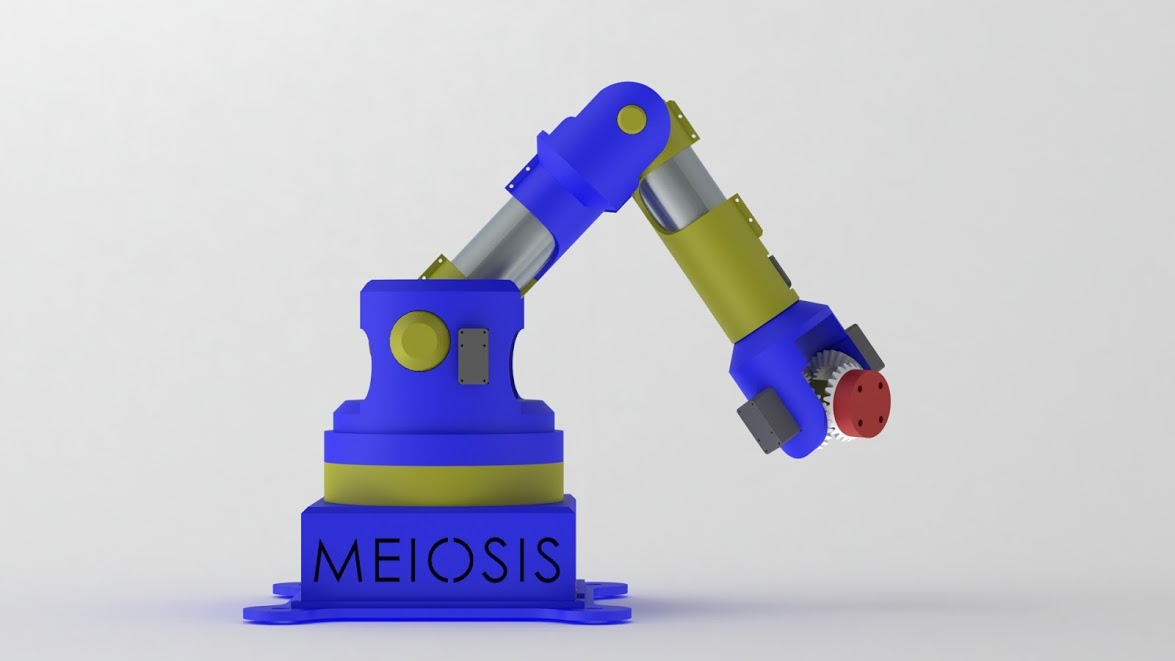
\includegraphics[width=.65\textwidth,frame]{concept1}
  \caption{First Conceptual Design}
  \label{fig:concept1}
\end{figure}
From Figure \ref{fig:concept1}, the manipulator included six rotational joints consisting of a base, shoulder, and elbow joint followed by a spherical wrist. The design used AX-12A smart servos to drive the joints, and a differential drive gearbox was placed in the wrist to decrease the size as well as improve the torque capabilities of the wrist. Aluminum tubing was also placed between the links to strengthen the manipulator. This conceptual design had its issues, however, creating the need for changes in the design, which can be seen in Figure \ref{fig:concept2}.
\begin{figure}[htp]
  \centering
  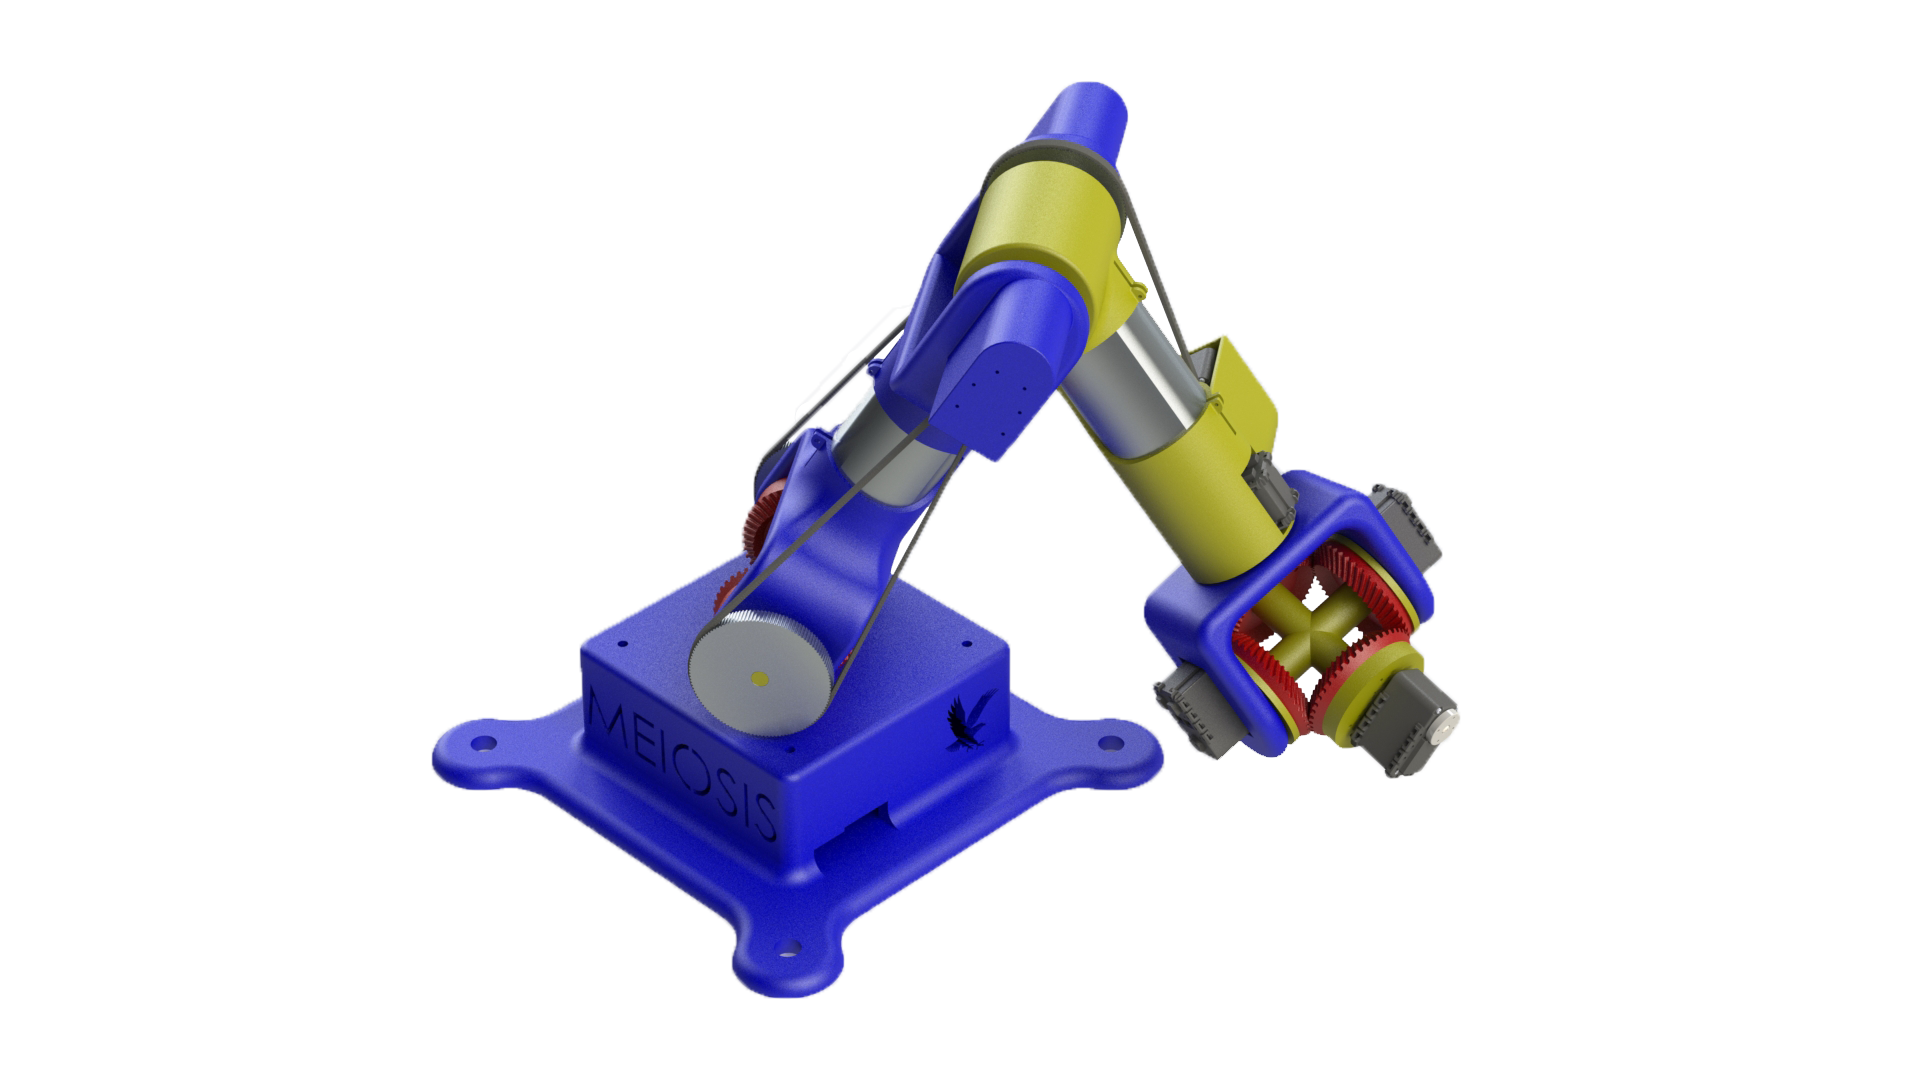
\includegraphics[width=.65\textwidth,frame]{concept2}
  \caption{Second Conceptual Design}
  \label{fig:concept2}
\end{figure}
Figure \ref{fig:concept2} shows that there were some drastic changes from the first conceptual design to the second design. All the servos on the manipulator were changed to the MX-12W as it was discovered that the AX-12A could not be used in the differential gearboxes as they had a sixty degree dead zone in which no usable data could be read. Since the MX-12W had lower torque output than the AX-12A, a differential gearbox replaced the first and second joints to share the load from the arm between two servos, and a belt system was implemented to help gear up the torque output from the servos as well as to lower the angle error of the servos. The third joint also received a belt system to help with the torque and angle precision. While there were more capable smart servos available for purchase, all servos that could be used with the differential without gearing would not have kept us within budget. This design, however, also had its own problems, prompting another redesign shown in Figure \ref{fig:MEIOSISFinalDesign}.
\begin{figure}[htp]
  \centering
  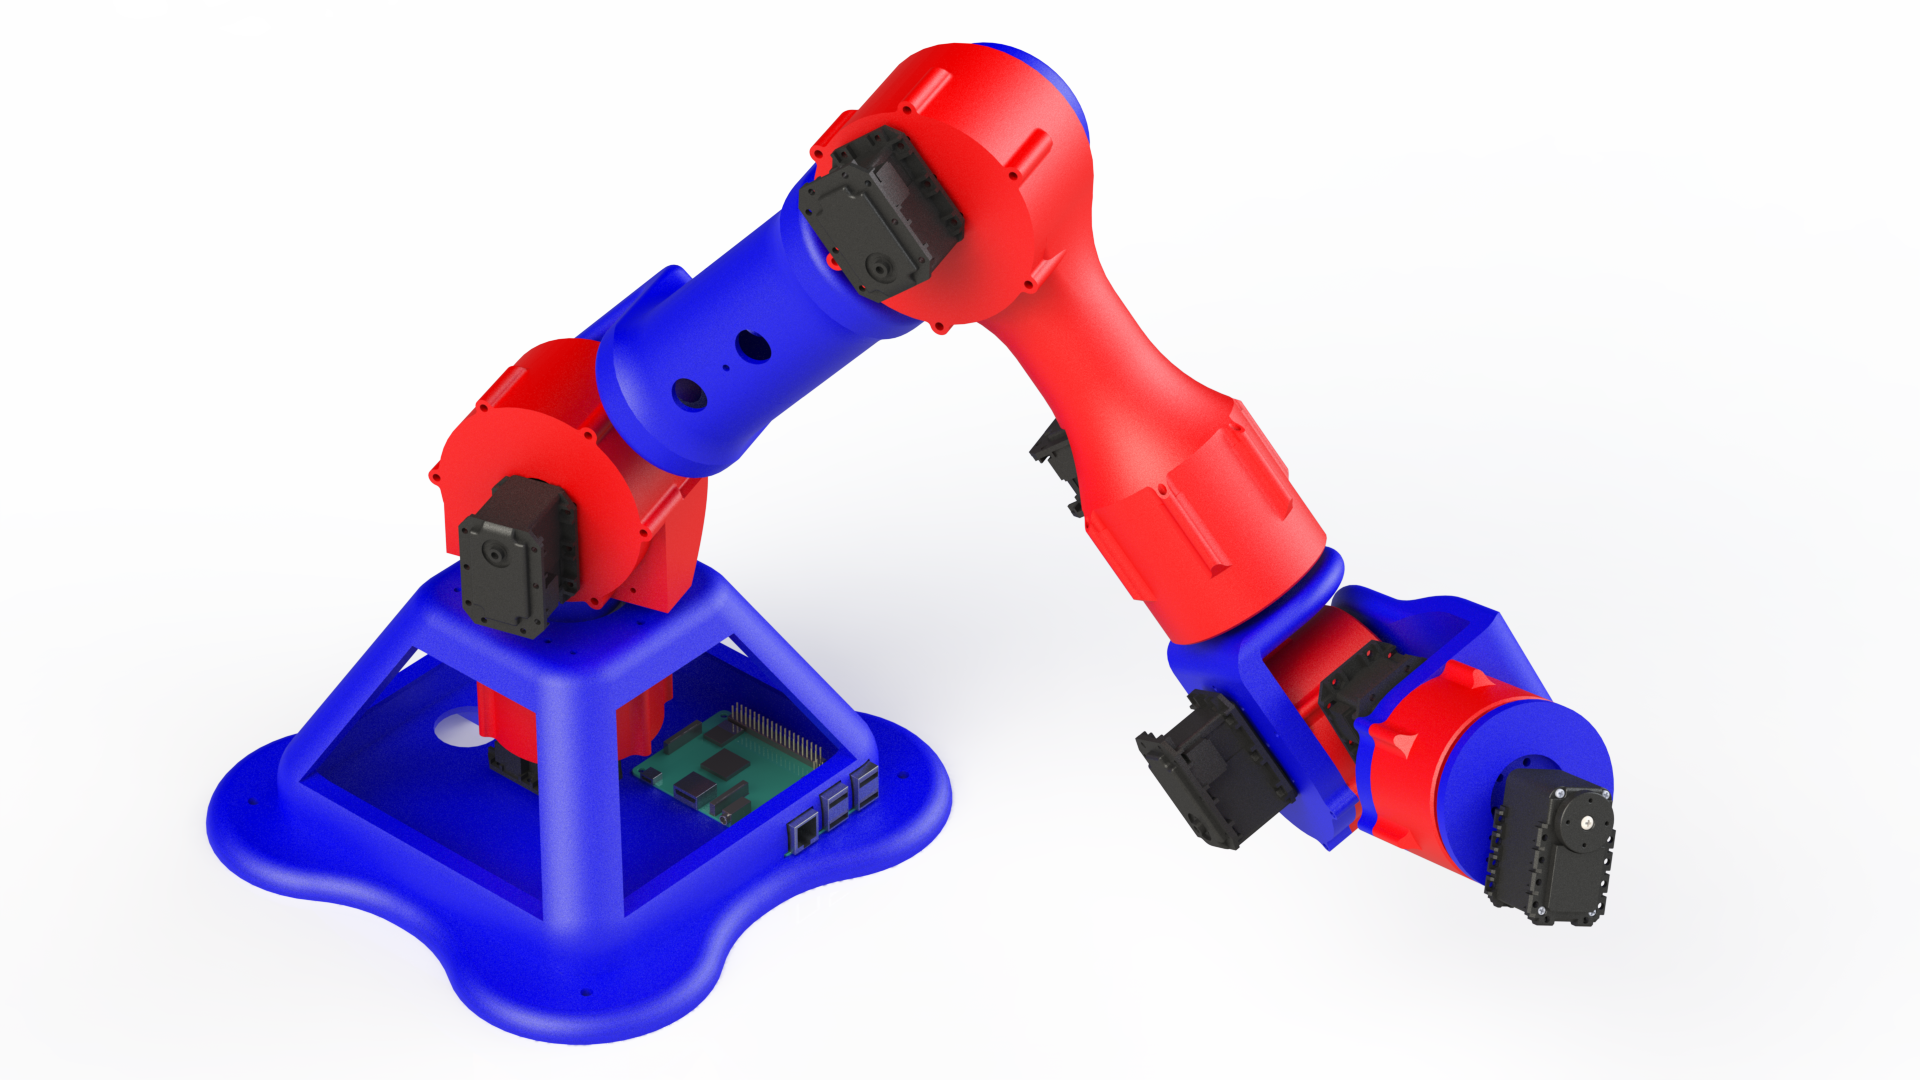
\includegraphics[width=.65\textwidth,frame]{MEIOSISFinalDesign}
  \caption{MEIOSIS Final Design}
  \label{fig:MEIOSISFinalDesign}
\end{figure}
Several design changes from the second conceptual design can be noted in Figure \ref{fig:MEIOSISFinalDesign}. The first major design change is changing the link material from a hybrid design to a fully 3D printed design. This change was made to reduce the overall weight of each link. Additionally, after Ansys stress testing, it was determined that using aluminum to make the links stronger was unnecessary. Reducing the link weights allows for lower gear ratios since the torque required to move each link is lower. The second major design change is utilizing a completely different power transmission system for the joints. As seen in \ref{fig:concept2}, the second design used a differential drive system, which allowed for the torque of joint two to be shared between two servos. The load distribution was necessary since the links were too heavy for a single MX-12W servo to lift. However, once a prototype of the differential drive system was created, it was determined that the backlash within the gears was too high to meet the required level of precision. The newest design features a harmonic gearbox on each joint, which allows for a much higher level of accuracy than the previous differential drive version. A 39:1 harmonic gearbox is used in the elbow and the shoulder as they face the highest loads, and a 20:1 harmonic gearbox is used in the remainder of the joints. The benefit of using a harmonic gearbox is that a high gear ratio can be achieved with very little internal backlash, negating both the need for the pulley system and the need to share the load between two servos. The servos in the first three joints were also changed from the MX-12W to the MX-64T to ensure that the servos would function at one fifth of their stall torque. Because the MX-64T servos are able to rotate plus or minus twenty-eight rotations, the servos are usable in the differential. Since the harmonic gearboxes are different in size compared to the differential, the link lengths in the end effector changed slightly. The base was also changed to reduce the amount of PLA material used.
